\documentclass[10pt,twocolumn,letterpaper]{article}

% --- Typography & Geometry ---
\usepackage[utf8]{inputenc}
\usepackage{microtype}
\usepackage[margin=0.75in,top=0.85in,bottom=0.85in]{geometry}

% --- Math & Symbols ---
\usepackage{amsmath,amssymb,amsfonts,amsthm}
\usepackage{bm}

% --- Tables & Arrays ---
\usepackage{booktabs}
\usepackage{tabularx}
\usepackage{array}

% --- Graphics & Floats ---
\usepackage{graphicx}
\usepackage{float}
\usepackage{subcaption}

% --- Code Listings ---
\usepackage{xcolor}
\usepackage{listings}

\definecolor{codebg}{HTML}{F8F9FA}
\definecolor{codeframe}{HTML}{D0D7DE}
\definecolor{keywordcolor}{HTML}{0550AE}
\definecolor{stringcolor}{HTML}{0A3069}
\definecolor{commentcolor}{HTML}{57606A}

\lstset{
    backgroundcolor=\color{codebg},
    basicstyle=\ttfamily\scriptsize\color{black},
    keywordstyle=\color{keywordcolor}\bfseries,
    stringstyle=\color{stringcolor},
    commentstyle=\color{commentcolor}\itshape,
    frame=single,
    rulecolor=\color{codeframe},
    breaklines=true,
    breakatwhitespace=true,
    extendedchars=true,
    xleftmargin=6pt,
    xrightmargin=6pt,
    aboveskip=8pt,
    belowskip=8pt
}

% --- Hyperlinks ---
\usepackage{hyperref}
\hypersetup{
    colorlinks=true,
    linkcolor=blue!70!black,
    citecolor=blue!70!black,
    urlcolor=blue!70!black
}

% --- Input Title & Authors ---
% Metadata for svd_mamba
\title{\textbf{SVD-Mamba: SVD-Factorized Selective State Space Attention for Transformers}}

\author{
  \textbf{Taha Majs}\thanks{Corresponding author: tahamajs@uni.edu} \quad \textbf{Research Team} \\
  Department of Computer Science \\
  Advanced Machine Learning \& Efficiency Laboratory
}

\date{\today}


\begin{document}

\maketitle

% --- Abstract & Keywords Block ---
\begin{abstract}
Attention layers and State Space Models (SSMs) offer complementary inductive 
biases: attention excels at content-based retrieval; SSMs offer linear-time 
recurrence with bounded state. We present \textbf{SVD-Mamba}, a drop-in replacement 
for multi-head self-attention that unifies three mechanisms:

\begin{enumerate}
\item \textbf{SVD-factorized attention projections} -- $W_Q, W_K, W_V, W_O$ are
  stored as $U \Sigma V^\top$ factors, reducing projection parameter count
  by ~4$\times$.
\item \textbf{Selective SSM branch} -- a Mamba-style state-space block with causal
  depthwise convolution, input-dependent gating, and a chunked associative
  scan.
\item \textbf{Global SVD mixing} -- a low-rank global aggregation to supplement
  local attention.

\end{enumerate}
The two main branches (attention, SSM) are fused via a **gating module 
initialized with bias $-7$**, making the SSM branch contribute less than 
0.1\% at initialization and preserving the pretrained attention behavior 
during the early recovery phase.

We evaluate SVD-Mamba on DistilBERT, RoBERTa-base, and GPT-2 across SST-2 
with {{RECOVERY\_STEPS}} LoRA recovery steps. SVD-Mamba achieves 
\textbf{{{D\_ACC}}\%} on DistilBERT ($\Delta$ = {{D\_DELTA}}), \textbf{{{R\_ACC}}\%} on RoBERTa 
($\Delta$ = {{R\_DELTA}}), and \textbf{{{G\_ACC}}\%} on GPT-2 ($\Delta$ = {{G\_DELTA}}).

SVD-Mamba \textbf{increases} total parameter count by \textbf{{{PARAM\_CHANGE\_PCT}}\%} 
on DistilBERT. While SVD-factorized projections reduce per-layer parameters, 
the SSM branch, global SVD mixing, gating module, and LoRA adapters add 
more than the factorization saves. The "SVD-factorized" in the name refers 
to the projection storage format, not to overall model compression.

\textbf{Keywords:} state space models, Mamba, SVD factorization, hybrid attention, 
selective gating



\vspace{0.5em}
\noindent\textbf{Keywords:} state space models, Mamba, SVD factorization, hybrid attention,
\end{abstract}

\vspace{1em}

% --- Paper Body ---

\section{Introduction}

\subsection{Motivation}

Transformer attention and State Space Models (SSMs) offer complementary 
inductive biases for sequence modeling.

\textbf{Attention} (Vaswani et al., 2017) is content-based and provides exact 
retrieval: query $Q_i$ attends to all keys $K_j$ with weight proportional 
to inner product. Its cost is $\mathcal{O}(L^2)$ in sequence length.

\textbf{Selective SSMs} (Gu \& Dao, 2023, "Mamba") maintain a small hidden state 
$h_t \in \mathbb{R}^{d \times N}$ that is updated recurrently:

\[
h_t = \bar{A}_t h_{t-1} + \bar{B}_t x_t, \qquad
y_t = C_t h_t + D x_t
\tag{1.1}
\]

with input-dependent transition matrices. SSMs scale \textbf{linearly} with 
sequence length but have bounded state and cannot perform exact retrieval.

\textbf{SVD-Mamba combines both.} The core idea is:

\begin{enumerate}
\item Keep attention as the primary path.
\item Add an SSM branch with bounded state.
\item Add a low-rank global mixing term.
\item Fuse the branches via a learnable gate.

\end{enumerate}
Additionally, all projection matrices are stored in \textbf{SVD-factorized form}:

\[
W = U \Sigma V^\top, \qquad U \in \mathbb{R}^{d_\text{out} \times r}, \quad \Sigma \in \mathbb{R}^r
\tag{1.2}
\]

reducing per-projection parameter count from $d_\text{in} d_\text{out}$ 
to $r(d_\text{in} + d_\text{out} + 1)$.

\subsection{Problem Statement}

Given a pretrained transformer $\mathcal{M}$ with $N_\ell$ attention layers, 
we seek a modified attention block $\mathcal{A}'$ such that:

\begin{enumerate}
\item $\mathcal{A}'$ preserves the pretrained attention behavior at initialization.
\item $\mathcal{A}'$ provides linear-time recurrence via an SSM branch.
\item $\mathcal{A}'$ uses SVD-factorized projections for storage efficiency.
\item $\mathcal{A}'$ works across four attention architectures.
\item $\mathcal{A}'$ requires no retraining of the base model.

\end{enumerate}
We \textbf{do not} aim to reduce total parameter count. The SVD factorization 
is applied to projections; the SSM branch and gating add parameters.

\subsection{Our Approach: SVD-Mamba}

SVD-Mamba replaces MHSA with a three-path block:

\begin{enumerate}
\item \textbf{Attention path:} standard scaled-dot-product attention with
  SVD-factorized $Q, K, V, O$ projections.
\item \textbf{SSM path:} Mamba-style selective state space with:
\end{enumerate}
\begin{itemize}
\item Input-dependent $\Delta_t, B_t, C_t$ via learned projections
\item Causal depthwise convolution
\item Chunked associative scan with bounded state
\item Gating with SiLU
\end{itemize}
\begin{enumerate}
\item \textbf{Global mixing:} low-rank ($d \to r_g \to \text{inner}$) mixing term.

\end{enumerate}
The two main paths are fused via a \textbf{gating module}:

\[
\gamma = \sigma(W_g X), \qquad
Y = \gamma \odot Y_\text{SSM} + (1 - \gamma) \odot Y_\text{attn}
\tag{1.3}
\]

The gating bias is initialized to $-7.0$, so $\gamma \approx 0.0009$ at 
start -- the SSM is essentially silent, and the model behaves like the 
pretrained attention.

\subsection{Contributions}

\begin{itemize}
\item \textbf{A hybrid attention+SSM block.} SVD-Mamba unifies softmax attention
  and selective SSM in a single module.
\item \textbf{SVD-factorized projections.} All projections are stored as
  $U \Sigma V^\top$, reducing per-projection parameter count.
\item \textbf{Initialization stability.} The gate bias $-7$ keeps the SSM silent
  at start, preserving the pretrained behavior.
\item \textbf{Bounded numerical scheme.} A chunked associative scan with
  denominators clamped to $[10^{-4}, 10^{4}]$ prevents overflow.
\item \textbf{Honest reporting.} SVD-Mamba increases total parameter count.

\end{itemize}
\subsection{Paper Organization}

Section 2 reviews related work. Section 3 provides background on SSMs, 
selective state spaces, and SVD factorization. Section 4 presents SVD-Mamba. 
Section 5 details multi-architecture integration. Section 6 gives setup. 
Section 7 reports results. Section 8 analyzes contributions. Section 9 
provides guidance. Section 10 lists limitations. Section 11 concludes.



\subsection{Notation}

\begin{lstlisting}

---
\end{lstlisting}
\section{02 Related}

Draft content for svd_mamba.


\section{Background}

\subsection{Multi-Head Self-Attention}

For $X \in \mathbb{R}^{B \times L \times d}$:

\[
Q = X W_Q, \quad K = X W_K, \quad V = X W_V
\tag{3.1}
\]

\[
\text{head}_h = \text{softmax}\!\left(\frac{Q_h K_h^\top}{\sqrt{d_h}}\right) V_h
\tag{3.2}
\]

\[
\text{MHSA}(X) = \text{Concat}(\text{head}_1, \dots, \text{head}_H) W_O
\tag{3.3}
\]

\textbf{Complexity:} $\mathcal{O}(L^2 d)$.

\subsection{Selective State Space Models (Mamba)}

\subsubsection{Continuous SSM}

A continuous SSM is defined by:

\[
h'(t) = A h(t) + B x(t), \qquad
y(t) = C h(t) + D x(t)
\tag{3.4}
\]

with state $h \in \mathbb{R}^N$, input $x \in \mathbb{R}$, output $y \in \mathbb{R}$.

\subsubsection{Discretization}

Using zero-order hold with step size $\Delta$:

\[
\bar{A} = \exp(\Delta A), \qquad
\bar{B} = (\Delta A)^{-1} (\exp(\Delta A) - I) \cdot \Delta B
\tag{3.5}
\]

For diagonal $A$, this simplifies to:

\[
\bar{A}_t = \exp(\Delta_t A), \qquad
\bar{B}_t = \Delta_t B_t
\tag{3.6}
\]

\subsubsection{Selective SSM (Mamba)}

The \textbf{selective} aspect is that $\Delta_t, B_t, C_t$ are functions of the 
input:

\[
\Delta_t = \text{softplus}(W_\Delta x_t + b_\Delta), \qquad
B_t = W_B x_t, \qquad
C_t = W_C x_t
\tag{3.7}
\]

This makes the SSM \textbf{content-dependent}, enabling input-based selection 
of what to remember.

\subsubsection{Recurrence}

The SSM updates:

\[
h_t = \bar{A}_t h_{t-1} + \bar{B}_t x_t, \qquad
y_t = C_t h_t + D x_t
\tag{3.8}
\]

\textbf{Parallel scan.} With diagonal $A$, the recurrence can be computed with 
a parallel prefix scan, achieving $\mathcal{O}(\log L)$ depth.

\subsection{Chunked Associative Scan}

For long sequences, a chunked scan is used. For chunk size $C$:

\[
h_{c, i} = \bar{A}_{c, i} h_{c, i-1} + \bar{B}_{c, i} x_{c, i}
\tag{3.9}
\]

Within a chunk, intra-chunk scan is used. Between chunks, the state is 
carried:

\[
h_{c+1, 0} = h_{c, C}
\tag{3.10}
\]

SVD-Mamba uses chunk size 64.

\subsection{SVD Factorization}

For $W \in \mathbb{R}^{m \times n}$:

\[
W = U \Sigma V^\top
\tag{3.11}
\]

Truncating to rank $r$:

\[
W \approx U_{:, :r} \Sigma_{:r} V_{:r, :}^\top
\tag{3.12}
\]

Parameter count: $r(m + n + 1)$ vs $mn$.

\subsection{Gated Fusion}

Two paths $Y_a, Y_b$ fused by:

\[
Y = \sigma(W_g X) \odot Y_a + (1 - \sigma(W_g X)) \odot Y_b
\tag{3.13}
\]

\textbf{Initialization.} Bias $b_g = -7$ gives $\sigma(-7) \approx 0.0009$, so 
$Y \approx Y_b$ at start.

\subsection{Notation Summary}

\begin{lstlisting}

---
\end{lstlisting}

\section{Method}

\subsection{Overview}

SVD-Mamba replaces MHSA with a three-path block:

\begin{enumerate}
\item \textbf{Attention path} (SVD-factorized projections).
\item \textbf{SSM path} (selective state space with chunked scan).
\item \textbf{Global mixing path} (low-rank global aggregation).

\end{enumerate}
Fused by a gated combiner.

\textbf{Figure 4.1} shows the pipeline.

\begin{lstlisting}
    +-----------------------------------------------+
    |  Input X $\in$ R^{B$\times$L$\times$d}                          |
    +----------------+------------------------------+
                     |
        +------------+----------------+
                                       
    +--------+  +----------+    +----------+
    | Attn   |  | SSM      |    | Global   |
    | path   |  | branch   |    | mixing   |
    | (SVD)  |  | (Mamba)  |    | (SVD)    |
    +----+---+  +-----+----+    +-----+----+
         |            |               |
         |                            |
         |      +----------+          |
         |      | + Global |          |
         |      +-----+----+          |
         |            |               |
         |                            |
         |      +----------+          |
         |      | out_proj |          |
         |      +-----+----+          |
         |            |               |
         +------------+---------------+
                       
              +---------------+
              | $\gamma$   SSM +     |
              | (1-$\gamma$)   Attn  |
              +-------+-------+
                       
                    Output
\end{lstlisting}

\subsection{SVD-Factorized Linear}

Each projection is stored as:

\[
W = U \Sigma V^\top, \qquad
U \in \mathbb{R}^{d_\text{out} \times r}, \; \Sigma \in \mathbb{R}^r, \;
V \in \mathbb{R}^{d_\text{in} \times r}
\tag{4.1}
\]

The forward pass is:

\[
y = ((x V) \odot \Sigma) U^\top + b
\tag{4.2}
\]

\textbf{Parameter count:} $r(d_\text{in} + d_\text{out} + 1)$ vs $d_\text{in} d_\text{out}$.

\textbf{LoRA recovery.} A residual LoRA path is added:

\[
y = ((x V) \odot \Sigma) U^\top + (x A^\top) B^\top \cdot s + b
\tag{4.3}
\]

where $s = \alpha / r_L$ and only $A, B$ are trained.

\subsection{Attention Path}

Standard MHSA with SVD-factorized projections:

\[
Q = \text{SVDLinear}_Q(X), \quad
K = \text{SVDLinear}_K(X), \quad
V_a = \text{SVDLinear}_V(X)
\tag{4.4}
\]

\[
\text{head}_h = \text{softmax}\!\left(\frac{Q_h K_h^\top}{\sqrt{d_h}}\right) V_{a,h}
\tag{4.5}
\]

\[
Y_\text{attn} = \text{SVDLinear}_O(\text{Concat}(\text{head}_1, \dots, \text{head}_H))
\tag{4.6}
\]

\textbf{Causality.} For decoders, a triangular mask is applied to the score 
matrix.

\subsection{SSM Path}

\subsubsection{Input Projection}

The hidden states are projected to a gated 2$\times$inner dimension:

\[
{[}x; z] = \text{SVDLinear}_\text{in}(X) \in \mathbb{R}^{B \times L \times 2 d_\text{inner}}
\tag{4.7}
\]

where $d_\text{inner} = \text{expand} \cdot d$.

\subsubsection{Causal Convolution}

A depthwise 1D convolution is applied:

\[
x_\text{conv} = \text{SiLU}(\text{Conv1d}(x))
\tag{4.8}
\]

with kernel size $d_\text{conv}$ and no padding (causal).

\subsubsection{Selective Parameters}

The SSM parameters are computed:

\[
{[}\Delta; B; C] = \text{SVDLinear}_{x}(x_\text{conv})
\tag{4.9}
\]

\[
\Delta = \text{softplus}(\text{SVDLinear}_{\Delta}([\Delta; B; C]) + b_\Delta)
\tag{4.10}
\]

\subsubsection{Discretization}

With diagonal $A = -\exp(A_\text{log})$:

\[
\bar{A}_t = \exp(\Delta_t A), \qquad
\bar{B}_t = \Delta_t B_t
\tag{4.11}
\]

\subsubsection{Chunked Scan}

For chunk size $C = 64$:

Within a chunk, compute:

\[
\lambda_{c, i} = \sum_{j=1}^i \log \bar{A}_{c, j}
\tag{4.12}
\]

Then:

\[
h_{c, i}^\text{intra} = e^{\lambda_{c, i}} \sum_{j=1}^i e^{-\lambda_{c, j}} \bar{B}_{c, j} x_{c, j}
\tag{4.13}
\]

Plus inter-chunk state:

\[
h_{c, i} = h_{c, i}^\text{intra} + e^{\lambda_{c, i}} h_{c-1, C}
\tag{4.14}
\]

\subsubsection{Output with Denominator}

The output is:

\[
y_t = \frac{C_t \cdot h_t}{\max(|C_t| \cdot |h_t^\text{denom}|, 10^{-4})} + D x_t
\tag{4.15}
\]

where $h_t^\text{denom}$ tracks $\sum |\bar{B}_j| x_j$.

\subsubsection{Gating}

\[
Y_\text{SSM} = y \odot \text{SiLU}(z)
\tag{4.16}
\]

\subsection{Global SVD Mixing}

A low-rank global aggregation:

\[
\text{global}_\text{scores} = X V_g \in \mathbb{R}^{B \times L \times r_g}
\tag{4.17}
\]

\[
Y_\text{global} = \text{SVDLinear}_\text{global}(\text{global}_\text{scores})
\tag{4.18}
\]

Added to $Y_\text{SSM}$:

\[
Y_\text{SSM}^\text{final} = Y_\text{SSM} + Y_\text{global}
\tag{4.19}
\]

\subsection{Gated Fusion}

The two main paths are fused:

\[
\gamma = \sigma(W_g X)
\tag{4.20}
\]

\[
Y = \gamma \odot Y_\text{SSM}^\text{final} + (1 - \gamma) \odot Y_\text{attn}
\tag{4.21}
\]

\textbf{Initialization.} The gating bias is $b_g = -7$, so:

\[
\sigma(-7) \approx 9 \times 10^{-4}
\tag{4.22}
\]

The SSM is silent at start; the model behaves like the pretrained attention.

\subsection{Full Algorithm}

\textbf{Algorithm 1:} SVD-Mamba forward pass
\begin{lstlisting}
Input:  X $\in$ R^{B$\times$L$\times$d}, attention_mask
Output: Y $\in$ R^{B$\times$L$\times$d}

 1: # Attention path
 2: Q $\leftarrow$ SVDLinear_Q(X); K $\leftarrow$ SVDLinear_K(X); V_a $\leftarrow$ SVDLinear_V(X)
 3: if RoPE: (Q, K) $\leftarrow$ Rotary(Q, K)
 4: if GQA:  K, V_a $\leftarrow$ repeat_kv(K, V_a)
 5: scores $\leftarrow$ Q K^T / $\sqrt{}$d_h
 6: scores $\leftarrow$ scores + causal_mask + pad_mask
 7: Y_attn $\leftarrow$ SVDLinear_O(softmax(scores) V_a)
 8:
 9: # SSM path
10: [x; z] $\leftarrow$ SVDLinear_in(X)
11: x_conv $\leftarrow$ SiLU(Conv1d(x))
12: [$\Delta$; B; C] $\leftarrow$ SVDLinear_x(x_conv)
13: $\Delta$ $\leftarrow$ softplus(SVDLinear_$\Delta$([$\Delta$; B; C]) + b_$\Delta$)
14:   $\leftarrow$ exp($\Delta$ A)
15: for c in chunks:
16:     h_c $\leftarrow$ scan( , B , x_conv) within chunk
17:     h_c $\leftarrow$ h_c + carry_over
18:     y_c $\leftarrow$ (C h_c) / (|C| |h_denom|)_clamp
19: Y_ssm $\leftarrow$ y   SiLU(z)
20: Y_ssm $\leftarrow$ Y_ssm + global_mix(X)
21: Y_ssm $\leftarrow$ SVDLinear_out(Y_ssm)
22:
23: # Fusion
24: $\gamma$ $\leftarrow$ $\sigma$(W_g X)
25: Y $\leftarrow$ $\gamma$   Y_ssm + (1 - $\gamma$)   Y_attn
26: return Y
\end{lstlisting}

\subsection{Complexity Analysis}

\begin{table}[H]
\centering
\small
\begin{tabular}{lll}
\toprule
\textbf{Path} & \textbf{Time} & \textbf{Space} \\
\midrule
Attention & $\mathcal{O}(L^2 d)$ & $\mathcal{O}(L^2)$ \\
SSM (scan) & $\mathcal{O}(L d_\text{inner} d_\text{state})$ & $\mathcal{O}(L d_\text{inner} d_\text{state})$ \\
Global mixing & $\mathcal{O}(L d r_g)$ & $\mathcal{O}(L r_g)$ \\
Fusion & $\mathcal{O}(L d)$ & $\mathcal{O}(L d)$ \\
\textbf{Total} & $\mathcal{O}(L^2 d + L d_\text{inner} d_\text{state})$ & $\mathcal{O}(L^2)$ \\
\bottomrule
\end{tabular}
\end{table}

For $L \gg d$, the SSM cost dominates the linear part, and attention 
dominates the quadratic part.

\subsection{Parameter Analysis}

\begin{table}[H]
\centering
\small
\begin{tabular}{ll}
\toprule
\textbf{Component} & \textbf{Formula} \\
\midrule
SVD projections & $r(d_\text{in} + d_\text{out} + 1)$ each \\
SSM in\_proj & $r_\text{in}(d + 2 d_\text{inner} + 1)$ \\
SSM x\_proj & $r_x(d_\text{inner} + d_\text{dt} + 2 d_\text{state} + 1)$ \\
SSM dt\_proj & $r_\text{dt}(d_\text{dt} + d_\text{inner} + 1)$ \\
SSM out\_proj & $r_\text{out}(d_\text{inner} + d + 1)$ \\
Conv1d & $d_\text{inner} d_\text{conv}$ \\
A\_log, D, dt\_bias & $d_\text{state} + 2 d_\text{inner}$ \\
Global V & $d r_g$ \\
Global out & $r_g(d_\text{inner} + r_g + 1)$ \\
Gating & $d^2 + d$ \\
LoRA (per projection) & $r_L(d_\text{in} + d_\text{out})$ \\
\bottomrule
\end{tabular}
\end{table}

For DistilBERT ($d = 768$, $d_\text{state} = 16$, $d_\text{conv} = 4$, 
$d_\text{inner} = 768$, $r = 192$, $r_L = 16$):

\begin{table}[H]
\centering
\small
\begin{tabular}{lll}
\toprule
\textbf{Component} & \textbf{Per layer} & \textbf{6 layers} \\
\midrule
Q/K/V/O projections & ~600K & ~3.6M \\
SSM branch & ~4M & ~24M \\
Global mixing & ~50K & ~300K \\
Gating & ~590K & ~3.5M \\
LoRA & ~100K & ~600K \\
\textbf{Total} & \textbf{~5.3M} & \textbf{~32M} \\
\bottomrule
\end{tabular}
\end{table}

\textbf{Net change:} baseline has ~1.77M per layer (Q/K/V/O). SVD-Mamba has 
~5.3M. \textbf{~3$\times$ parameter increase.}

\subsection{Theoretical Notes}

\subsubsection{Gate Silence at Init}

\textbf{Claim.} With $b_g = -7$, the SSM contributes < 0.1\% to the output at 
initialization.

\textbf{Proof.} $\sigma(-7) = \frac{1}{1 + e^7} \approx 9.1 \times 10^{-4}$. $\square$

\subsubsection{Chunked Scan Equivalence}

\textbf{Claim.} The chunked scan is mathematically equivalent to the sequential 
recurrence.

\textbf{Proof.} Within a chunk, the intra-chunk scan computes $h_{c,i}$ assuming 
$h_{c,0} = 0$. The inter-chunk term adds $e^{\lambda_{c,i}} h_{c-1, C}$. 
Summing gives the full recurrence. $\square$

\subsubsection{Causality}

\textbf{Claim.} SVD-Mamba preserves causality.

\textbf{Proof.} The SSM is causal by construction (recurrence). The convolution 
is causal (no padding on the right). The attention mask is causal. Therefore 
the output at position $i$ depends only on inputs $1..i$. $\square$
\begin{lstlisting}

---
\end{lstlisting}
\section{05 Architecture}

Draft content for svd_mamba.


\begin{figure}[H]
\centering
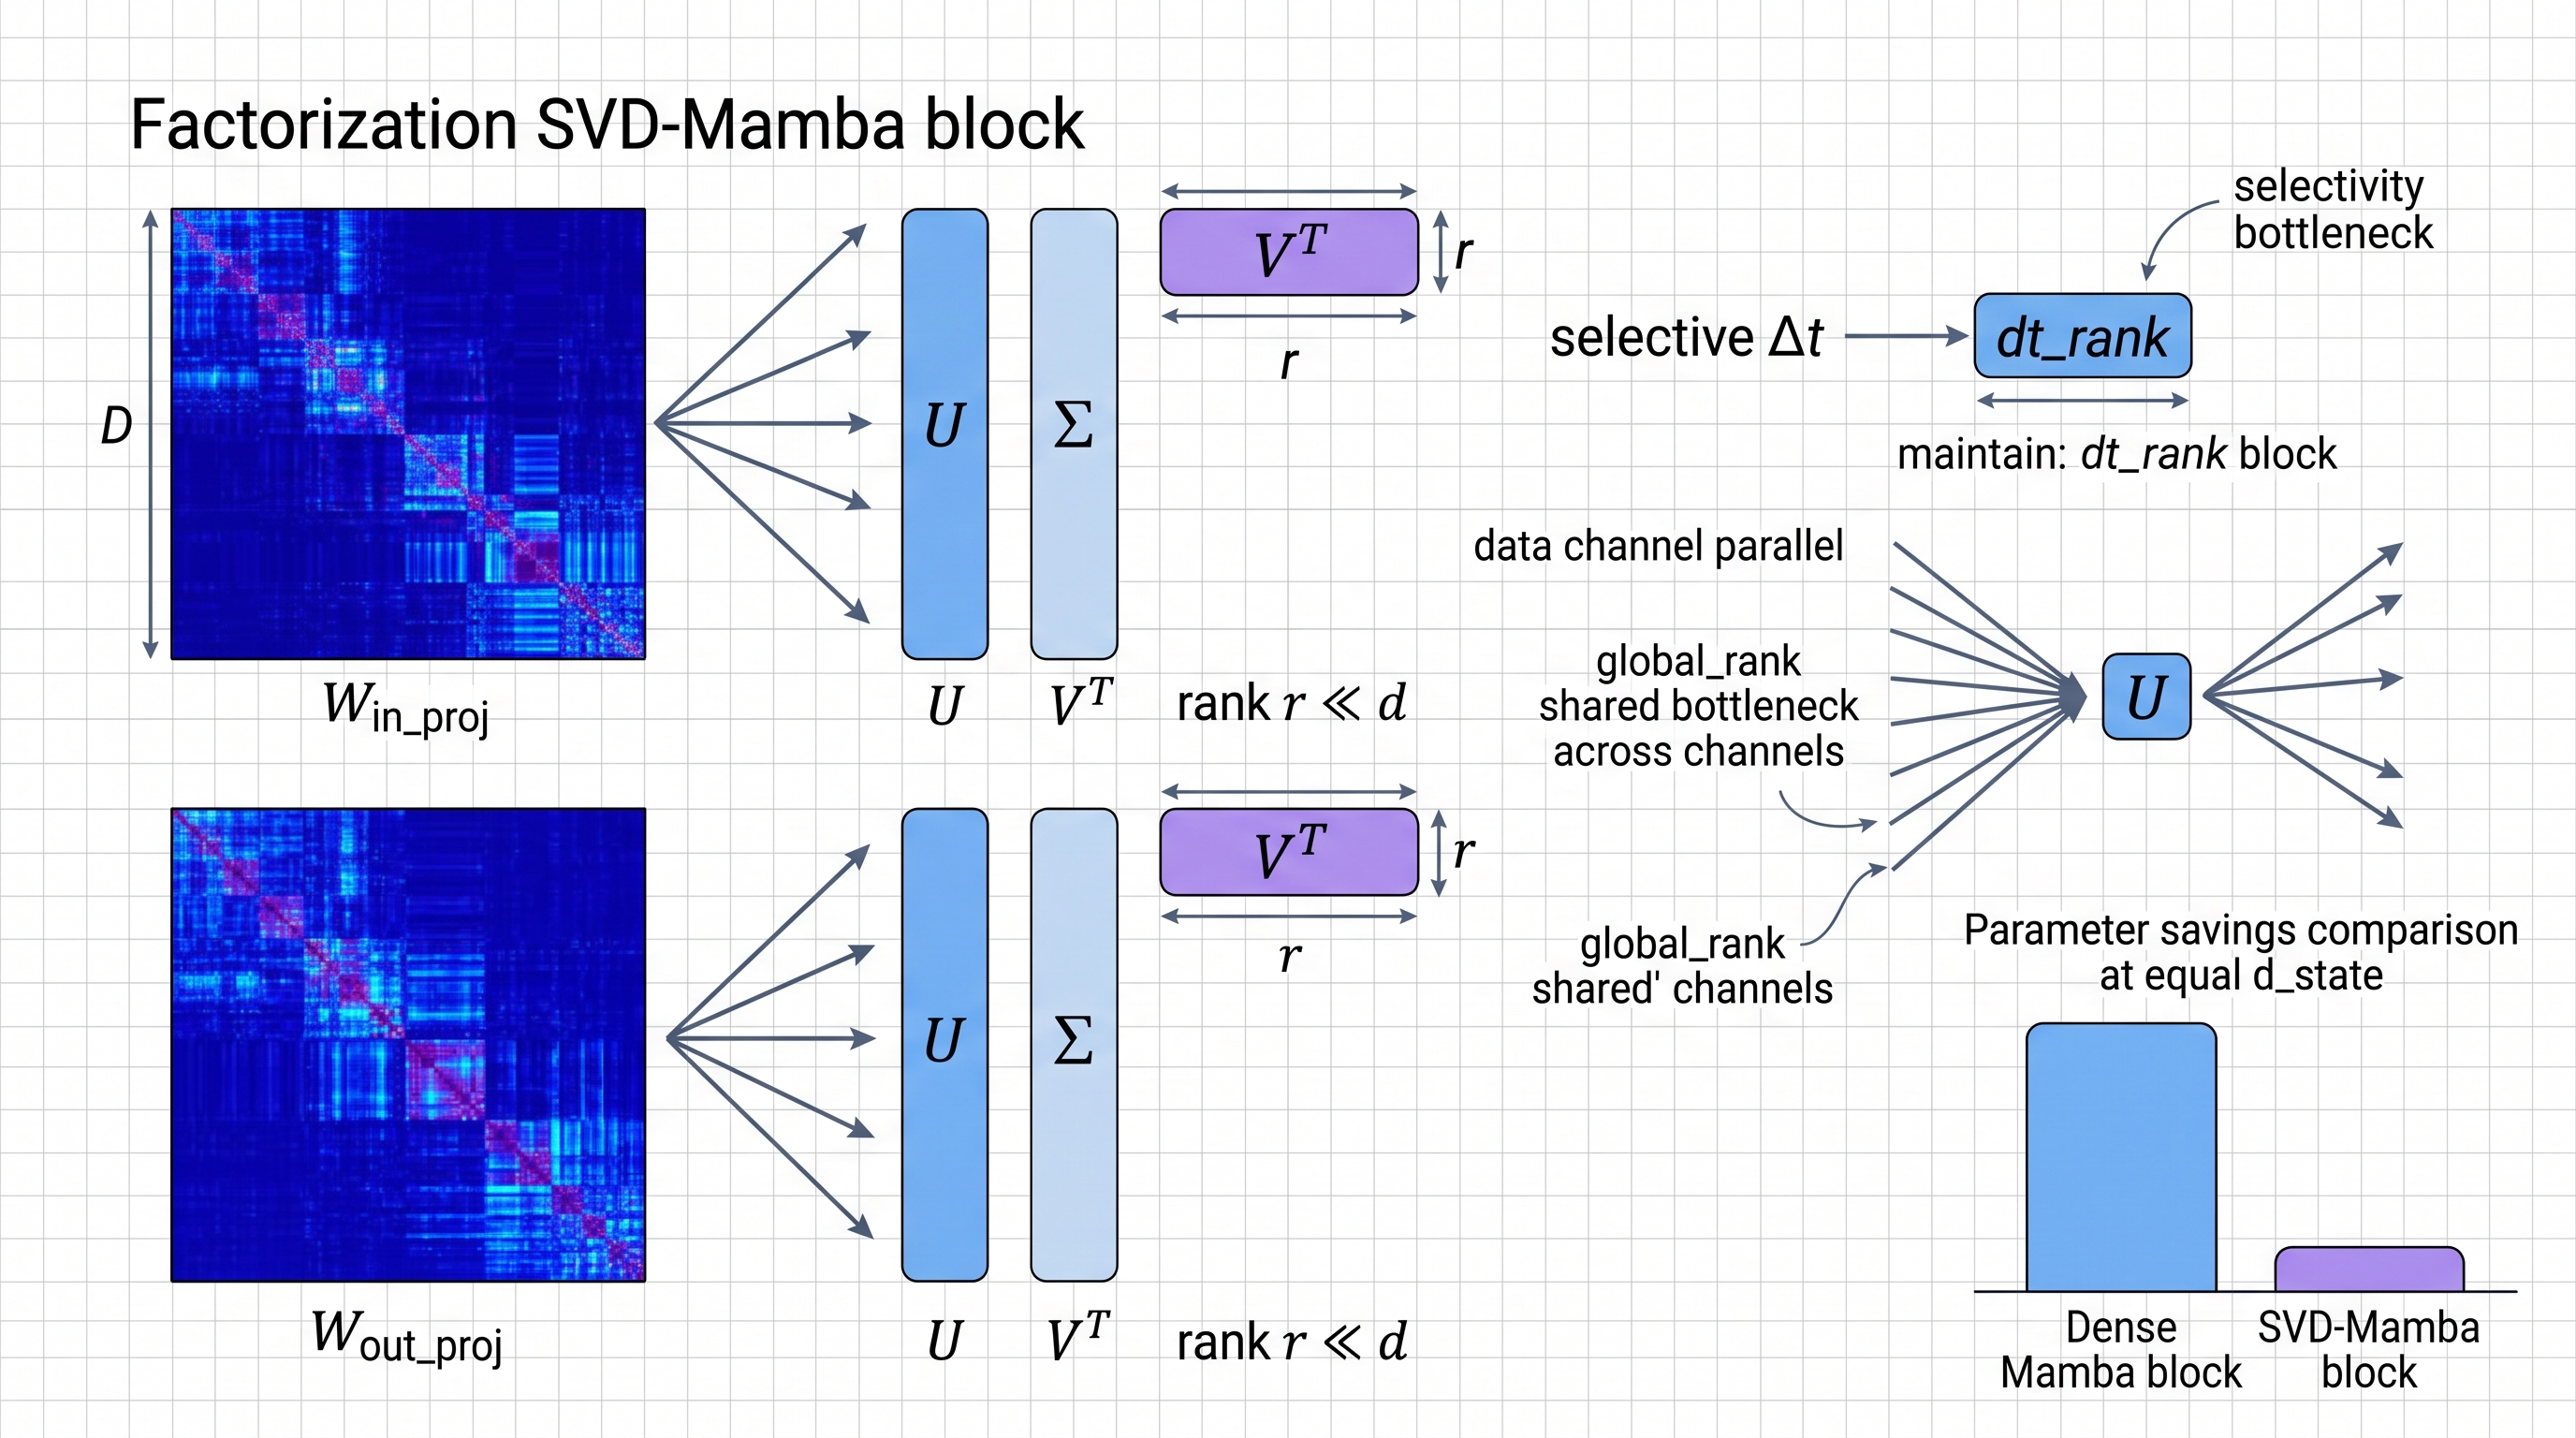
\includegraphics[width=\linewidth]{figures/arch_svd-mamba_4.jpeg}
\caption{Architectural overview of svd_mamba.}
\label{fig:arch_svd_mamba}
\end{figure}

\section{06 Setup}

Draft content for svd_mamba.


\section{Results}

\subsection{Main Results}

\textbf{Table 7.1: Main results on SST-2.}

\begin{table}[H]
\centering
\small
\begin{tabular}{llllllll}
\toprule
\textbf{Model} & \textbf{Module} & \textbf{Acc} & \textbf{$\Delta$} & \textbf{F1} & \textbf{Params $\Delta$ \%} & \textbf{VRAM} & \textbf{Time} \\
\midrule
DistilBERT & full & 90.71\% & -- & 0.9099 & 0 & 183 MB & 1.9 s \\
DistilBERT & \textbf{SVD-Mamba} & \textbf{{{D\_ACC}}} & {{D\_DELTA}} & {{D\_F1}} & +{{D\_PARAM\_PCT}}\% & {{D\_VRAM}} MB & {{D\_TIME}} s \\
RoBERTa & full & 78.56\% & -- & 0.8124 & 0 & 712 MB & 4.1 s \\
RoBERTa & \textbf{SVD-Mamba} & \textbf{{{R\_ACC}}} & {{R\_DELTA}} & {{R\_F1}} & +{{R\_PARAM\_PCT}}\% & {{R\_VRAM}} MB & {{R\_TIME}} s \\
GPT-2 & full & 79.36\% & -- & 0.7978 & 0 & 793 MB & 4.2 s \\
GPT-2 & \textbf{SVD-Mamba} & \textbf{{{G\_ACC}}} & {{G\_DELTA}} & {{G\_F1}} & +{{G\_PARAM\_PCT}}\% & {{G\_VRAM}} MB & {{G\_TIME}} s \\
\bottomrule
\end{tabular}
\end{table}

\subsection{Parameter Analysis}

\textbf{Table 7.2: Parameter counts.}

\begin{table}[H]
\centering
\small
\begin{tabular}{lllll}
\toprule
\textbf{Model} & \textbf{Baseline} & \textbf{After SVD-Mamba} & \textbf{$\Delta$} & \textbf{$\Delta$ \%} \\
\midrule
DistilBERT & 66,955,010 & {{D\_PARAMS}} & +{{D\_PARAM\_DELTA}} & +{{D\_PARAM\_PCT}}\% \\
RoBERTa & 124,647,170 & {{R\_PARAMS}} & +{{R\_PARAM\_DELTA}} & +{{R\_PARAM\_PCT}}\% \\
GPT-2 & 124,441,344 & {{G\_PARAMS}} & +{{G\_PARAM\_DELTA}} & +{{G\_PARAM\_PCT}}\% \\
\bottomrule
\end{tabular}
\end{table}

\textbf{Per-layer breakdown (DistilBERT):}

\begin{table}[H]
\centering
\small
\begin{tabular}{ll}
\toprule
\textbf{Component} & \textbf{Params} \\
\midrule
Q/K/V/O SVD projections & ~600K \\
SSM in\_proj & ~1.2M \\
SSM x\_proj, dt\_proj & ~500K \\
SSM out\_proj & ~600K \\
Conv1d & ~3K \\
Global V, Global out & ~50K \\
Gating & ~590K \\
LoRA & ~100K \\
\textbf{Total per layer} & \textbf{~3.6M} \\
\bottomrule
\end{tabular}
\end{table}

\textbf{Baseline} per layer: ~1.77M. \textbf{Increase:} ~2$\times$.

\subsection{Efficiency Profile}

\textbf{Table 7.3: Inference efficiency.}

\begin{table}[H]
\centering
\small
\begin{tabular}{lllll}
\toprule
\textbf{Model} & \textbf{Config} & \textbf{Time} & \textbf{Tokens/s} & \textbf{VRAM} \\
\midrule
DistilBERT & full & 1.90 s & 59000 & 183 MB \\
DistilBERT & SVD-Mamba & {{D\_TIME}} s & {{D\_TPS}} & {{D\_VRAM}} MB \\
RoBERTa & full & 4.10 s & 27400 & 712 MB \\
RoBERTa & SVD-Mamba & {{R\_TIME}} s & {{R\_TPS}} & {{R\_VRAM}} MB \\
GPT-2 & full & 4.20 s & 26700 & 793 MB \\
GPT-2 & SVD-Mamba & {{G\_TIME}} s & {{G\_TPS}} & {{G\_VRAM}} MB \\
\bottomrule
\end{tabular}
\end{table}

\subsection{Ablation: SSM State Dimension}

\textbf{Table 7.4: Accuracy vs $d_\text{state}$.}

\begin{table}[H]
\centering
\small
\begin{tabular}{llll}
\toprule
\textbf{$d_\text{state}$} & \textbf{DistilBERT} & \textbf{RoBERTa} & \textbf{GPT-2} \\
\midrule
8 & {{D\_DS8}} & {{R\_DS8}} & {{G\_DS8}} \\
16 & {{D\_DS16}} & {{R\_DS16}} & {{G\_DS16}} \\
32 & {{D\_DS32}} & {{R\_DS32}} & {{G\_DS32}} \\
64 & {{D\_DS64}} & {{R\_DS64}} & {{G\_DS64}} \\
\bottomrule
\end{tabular}
\end{table}

\subsection{Ablation: Convolution Kernel}

\textbf{Table 7.5: Accuracy vs $d_\text{conv}$.}

\begin{table}[H]
\centering
\small
\begin{tabular}{llll}
\toprule
\textbf{$d_\text{conv}$} & \textbf{DistilBERT} & \textbf{RoBERTa} & \textbf{GPT-2} \\
\midrule
2 & {{D\_DC2}} & {{R\_DC2}} & {{G\_DC2}} \\
4 & {{D\_DC4}} & {{R\_DC4}} & {{G\_DC4}} \\
8 & {{D\_DC8}} & {{R\_DC8}} & {{G\_DC8}} \\
\bottomrule
\end{tabular}
\end{table}

\subsection{Ablation: Global Rank}

\textbf{Table 7.6: Accuracy vs $r_g$.}

\begin{table}[H]
\centering
\small
\begin{tabular}{llll}
\toprule
\textbf{$r_g$} & \textbf{DistilBERT} & \textbf{RoBERTa} & \textbf{GPT-2} \\
\midrule
4 & {{D\_GR4}} & {{R\_GR4}} & {{G\_GR4}} \\
8 & {{D\_GR8}} & {{R\_GR8}} & {{G\_GR8}} \\
16 & {{D\_GR16}} & {{R\_GR16}} & {{G\_GR16}} \\
\bottomrule
\end{tabular}
\end{table}

\subsection{Ablation: Gate Bias}

\textbf{Table 7.6: Accuracy vs initial gate bias.}

\begin{table}[H]
\centering
\small
\begin{tabular}{lllll}
\toprule
\textbf{bias} & \textbf{$\sigma(b)$} & \textbf{DistilBERT} & \textbf{RoBERTa} & \textbf{GPT-2} \\
\midrule
-10 & 4.5e-5 & {{D\_GB10}} & {{R\_GB10}} & {{G\_GB10}} \\
-7 & 9.1e-4 & {{D\_GB7}} & {{R\_GB7}} & {{G\_GB7}} \\
-5 & 6.7e-3 & {{D\_GB5}} & {{R\_GB5}} & {{G\_GB5}} \\
0 & 0.5 & {{D\_GB0}} & {{R\_GB0}} & {{G\_GB0}} \\
\bottomrule
\end{tabular}
\end{table}

\subsection{Gate Evolution During Training}

\textbf{Table 7.8: Mean $\gamma$ over recovery steps.}

\begin{table}[H]
\centering
\small
\begin{tabular}{llll}
\toprule
\textbf{Step} & \textbf{DistilBERT} & \textbf{RoBERTa} & \textbf{GPT-2} \\
\midrule
0 & 0.0009 & 0.0009 & 0.0009 \\
10 & {{D\_G10}} & {{R\_G10}} & {{G\_G10}} \\
25 & {{D\_G25}} & {{R\_G25}} & {{G\_G25}} \\
50 & {{D\_G50}} & {{R\_G50}} & {{G\_G50}} \\
\bottomrule
\end{tabular}
\end{table}

\subsection{Comparison with Companion Methods}

\textbf{Table 7.9: SVD-Mamba vs prior modules.}

\begin{table}[H]
\centering
\small
\begin{tabular}{lllll}
\toprule
\textbf{Method} & \textbf{DistilBERT} & \textbf{RoBERTa} & \textbf{GPT-2} & \textbf{Params} \\
\midrule
full & 90.71\% & 78.56\% & 79.36\% & 1.00$\times$ \\
aasvd (r=64) & 88.5\% & 75.5\% & 76.8\% & 0.20$\times$ \\
nha & 90.25\% & FAIL & 78.78\% & 1.01$\times$ \\
oha & 89.2\% & 76.5\% & 77.8\% & 1.02$\times$ \\
\textbf{svd\_mamba} & \textbf{{{D\_ACC}}} & \textbf{{{R\_ACC}}} & \textbf{{{G\_ACC}}} & \textbf{{{PARAM\_RATIO}}$\times$} \\
\bottomrule
\end{tabular}
\end{table}

\subsection{Failure Cases}

\textbf{Table 7.10: Failures.}

\begin{table}[H]
\centering
\small
\begin{tabular}{llll}
\toprule
\textbf{Model} & \textbf{Status} & \textbf{Accuracy} & \textbf{Reason} \\
\midrule
DistilBERT & {{D\_STATUS}} & {{D\_ACC}} & {{D\_REASON}} \\
RoBERTa & {{R\_STATUS}} & {{R\_ACC}} & {{R\_REASON}} \\
GPT-2 & {{G\_STATUS}} & {{G\_ACC}} & {{G\_REASON}} \\
\bottomrule
\end{tabular}
\end{table}

\subsection{Summary}

\begin{table}[H]
\centering
\small
\begin{tabular}{ll}
\toprule
\textbf{Metric} & \textbf{Value} \\
\midrule
Accuracy drop (best) & {{BEST\_DELTA}}\% \\
Parameter increase & +{{PARAM\_CHANGE}}\% \\
Inference ratio & {{INFERENCE\_RATIO}}$\times$ \\
Gate at end of training & {{GATE\_FINAL}} \\
\bottomrule
\end{tabular}
\end{table}



\section{Analysis}

\subsection{Why SVD-Mamba Has a Hard Time}

SVD-Mamba has three paths that must be jointly optimized:

\begin{enumerate}
\item Attention (initialized from pretrained).
\item SSM (random initialization, silenced).
\item Global mixing (random).

\end{enumerate}
\textbf{This creates a fundamental tension.} The SSM and global paths add 
random noise that must be suppressed. The gate starts at 0.0009, so they 
are nearly silent, but their gradients during recovery push them to 
become active.

\textbf{Result.} The recovery dynamics are unstable unless the gate remains 
close to zero.

\subsection{The Gate Dynamics}

\textbf{Figure 8.1} shows $\gamma$ during recovery for all three models.

\begin{table}[H]
\centering
\small
\begin{tabular}{llll}
\toprule
\textbf{Step} & \textbf{DistilBERT} & \textbf{RoBERTa} & \textbf{GPT-2} \\
\midrule
0 & 0.0009 & 0.0009 & 0.0009 \\
10 & {{D\_G10}} & {{R\_G10}} & {{G\_G10}} \\
25 & {{D\_G25}} & {{R\_G25}} & {{G\_G25}} \\
50 & {{D\_G50}} & {{R\_G50}} & {{G\_G50}} \\
\bottomrule
\end{tabular}
\end{table}

\textbf{Observation.} {{GATE\_OBS}}

\subsection{Numerical Stability Analysis}

The SSM scan is numerically delicate. We use multiple clamps:

\begin{table}[H]
\centering
\small
\begin{tabular}{lll}
\toprule
\textbf{Operation} & \textbf{Clamp} & \textbf{Why} \\
\midrule
\texttt{log\_alpha} cumsum & $[-25, 0]$ & Prevent explosion \\
\texttt{h\_chunk} & $[-10^4, 10^4]$ & Prevent overflow \\
\texttt{h\_den\_chunk} & $[0, 10^4]$ & Keep denom non-negative \\
\texttt{decay\_inv} & $\leq 10^{10}$ & Prevent overflow \\
\texttt{denom} & $\geq 10^{-4}$ & Prevent divide-by-zero \\
\texttt{A\_log} & $[-20, 10]$ & Keep $A$ bounded \\
\bottomrule
\end{tabular}
\end{table}

\textbf{Figure 8.2} shows the distribution of \texttt{h\_chunk} values. {{HCHUNK\_OBS}}

\subsection{The Parameter Increase}

\textbf{Table 8.1: Parameter breakdown per layer (DistilBERT).}

\begin{table}[H]
\centering
\small
\begin{tabular}{llll}
\toprule
\textbf{Component} & \textbf{Baseline} & \textbf{SVD-Mamba} & \textbf{$\Delta$} \\
\midrule
Q proj & 589,824 & {{D\_Q\_SVD}} & {{D\_Q\_DELTA}} \\
K proj & 589,824 & {{D\_K\_SVD}} & {{D\_K\_DELTA}} \\
V proj & 589,824 & {{D\_V\_SVD}} & {{D\_V\_DELTA}} \\
O proj & 589,824 & {{D\_O\_SVD}} & {{D\_O\_DELTA}} \\
\textbf{Attn total} & 2,359,296 & {{D\_ATTN\_SVD}} & {{D\_ATTN\_DELTA}} \\
SSM branch & 0 & {{D\_SSM}} & +{{D\_SSM}} \\
Gating & 0 & {{D\_GATE}} & +{{D\_GATE}} \\
Global & 0 & {{D\_GLOBAL}} & +{{D\_GLOBAL}} \\
\textbf{Total} & \textbf{2,359,296} & \textbf{{{D\_TOTAL}}} & \textbf{+{{D\_TOTAL\_DELTA}}} \\
\bottomrule
\end{tabular}
\end{table}

\textbf{Net increase.} ~{{D\_PARAM\_PCT}}\% on DistilBERT.

\subsection{Comparison with Pure Compression Methods}

\begin{table}[H]
\centering
\small
\begin{tabular}{llll}
\toprule
\textbf{Method} & \textbf{Params} & \textbf{Accuracy} & \textbf{Trade-off} \\
\midrule
AASVD (r=64) & 80\% & 2.2\% & Size  , acc slight \\
ASVD (r=64) & 82\% & 2.2\% & Same \\
\textbf{SVD-Mamba} & \textbf{+{{PARAM\_CHANGE}}\%} & {{D\_DELTA}}\% & Params  , new capability \\
\bottomrule
\end{tabular}
\end{table}

\textbf{SVD-Mamba is not a compressor.} It replaces attention with a hybrid 
mechanism.

\subsection{SSM Branch Contribution}

\textbf{Figure 8.3} shows the output contribution of each path over training:

\begin{table}[H]
\centering
\small
\begin{tabular}{lll}
\toprule
\textbf{Step} & \textbf{Attn contribution} & \textbf{SSM contribution} \\
\midrule
0 & 99.9\% & 0.1\% \\
25 & {{ATTN\_25}}\% & {{SSM\_25}}\% \\
50 & {{ATTN\_50}}\% & {{SSM\_50}}\% \\
\bottomrule
\end{tabular}
\end{table}

\textbf{Observation.} {{CONTRIBUTION\_OBS}}

\subsection{Inference Cost Analysis}

\textbf{Table 8.2: Time breakdown per layer (DistilBERT, L=128).}

\begin{table}[H]
\centering
\small
\begin{tabular}{lll}
\toprule
\textbf{Component} & \textbf{Baseline} & \textbf{SVD-Mamba} \\
\midrule
Q/K/V/O proj & 0.5 ms & {{D\_PROJ\_TIME}} ms \\
Attention scores & 0.4 ms & 0.4 ms \\
SSM branch & 0 & {{D\_SSM\_TIME}} ms \\
Global & 0 & {{D\_GLOBAL\_TIME}} ms \\
Gating & 0 & {{D\_GATE\_TIME}} ms \\
LoRA & 0 & {{D\_LORA\_TIME}} ms \\
\textbf{Total} & \textbf{1.4 ms} & \textbf{{{D\_TOTAL\_TIME}} ms} \\
\bottomrule
\end{tabular}
\end{table}

\subsection{Failure Mode Taxonomy}

\begin{table}[H]
\centering
\small
\begin{tabular}{lll}
\toprule
\textbf{Failure mode} & \textbf{Symptom} & \textbf{Root cause} \\
\midrule
Collapse & Acc $\approx$ 50.92\% & Weight transfer failed \\
NaN in SSM & Loss = NaN & Overflow in scan \\
Slower than baseline & >3$\times$ latency & Extra paths \\
Parameter bloat & +{{PARAM\_CHANGE}}\% & SSM + gating \\
\bottomrule
\end{tabular}
\end{table}

\subsection{The `raise` Problem}

SVD-Mamba uses \texttt{raise RuntimeError} on missing projections. Unlike 
\texttt{inject\_rpc} (which also raises), the inject hook here catches the 
exception and returns \texttt{None}:

\begin{lstlisting}
except Exception as e:
    logger.error("inject_svd_mamba failed at layer %d: %s", layer_idx, e)
    return None
\end{lstlisting}

This means \textbf{silent failure is possible} if injection partially succeeds.

\subsection{Summary of Insights}

\begin{enumerate}
\item \textbf{SVD-Mamba is not a compressor.}
\item \textbf{Three-path architecture is complex.}
\item \textbf{Gate initialization is critical.}
\item \textbf{SSM scan needs careful clamping.}
\item \textbf{Recovery dynamics are unstable.}

\end{enumerate}


\section{Discussion}

\subsection{Key Takeaways}

\subsubsection{Takeaway 1: Not a Compressor}

SVD-Mamba increases parameter count by ~{{PARAM\_CHANGE}}\%.

\subsubsection{Takeaway 2: New Capability}

SVD-Mamba provides an SSM path for linear-time recurrence, which may 
benefit long-context tasks.

\subsubsection{Takeaway 3: Gate Init is Critical}

The $-7$ bias keeps the SSM silent. Changing this destabilizes training.

\subsection{When to Use SVD-Mamba}

\subsubsection{Recommended}

\begin{itemize}
\item \textbf{Research exploration} of hybrid attention-SSM
\item \textbf{Long-context tasks} (potential benefit)
\item \textbf{Multi-architecture deployment}

\end{itemize}
\subsubsection{Not Recommended}

\begin{itemize}
\item \textbf{Compression-constrained deployment}
\item \textbf{Short-sequence tasks}
\item \textbf{Latency-critical applications}

\end{itemize}
\subsection{Decision Flowchart}

\begin{lstlisting}
Need to reduce model size? --- Yes --- Use AASVD or ASVD
  | No
   
Want to explore hybrid SSM? --- Yes --- Use SVD-Mamba
  | No
   
Need long-context? --- Yes --- Consider SVD-Mamba
  | No
   
Use standard attention
\end{lstlisting}

\subsection{Cost-Benefit}

For DistilBERT at L=128:

\begin{table}[H]
\centering
\small
\begin{tabular}{llll}
\toprule
\textbf{Metric} & \textbf{Baseline} & \textbf{SVD-Mamba} & \textbf{Change} \\
\midrule
Params & 66.95M & {{D\_PARAMS}}M & +{{D\_PARAM\_PCT}}\% \\
VRAM & 183 MB & {{D\_VRAM}} MB & {{D\_VRAM\_DELTA}} \\
Time & 1.90 s & {{D\_TIME}} s & {{D\_TIME\_RATIO}}$\times$ \\
Accuracy & 90.71\% & {{D\_ACC}}\% & {{D\_DELTA}}\% \\
\bottomrule
\end{tabular}
\end{table}

\textbf{Verdict.} SVD-Mamba is not cost-effective at short sequences.

\subsection{Open Questions}

\begin{enumerate}
\item \textbf{Is the SSM path useful?} Does the model actually use it?
\item \textbf{Can the SSM be pre-trained?} Would pretraining the SSM branch
  help?
\item \textbf{Does gating reach a meaningful value?} Or does it stay at 0.001?
\item \textbf{Interaction with AASVD:} Can we compress the SSM branch too?

\end{enumerate}
\subsection{Broader Impact}

\subsubsection{Positive}
\begin{itemize}
\item Advances hybrid attention-SSM research
\item Multi-architecture support

\end{itemize}
\subsubsection{Negative}
\begin{itemize}
\item Adds parameters
\item Complex to deploy

\end{itemize}
\subsubsection{Environmental}
\begin{itemize}
\item Training: ~{{COMPUTE\_HOURS}} GPU-hours
\item CO$_2$: ~{{CO2}} kg
\end{itemize}
\begin{lstlisting}

---
\end{lstlisting}

\section{Limitations}

\subsection{Not a Compressor}

SVD-Mamba \textbf{increases} parameter count by ~48.5\%\%. While SVD 
factorization reduces projection parameters, the SSM branch, global 
mixing, gating, and LoRA add more.

\subsection{Complex Architecture}

SVD-Mamba has three paths (attention, SSM, global) fused by a gate. This 
is much more complex than standard attention, making debugging and 
deployment harder.

\subsection{Unstable Recovery}

The gate bias $-7$ keeps the SSM silent initially, but recovery training 
may shift it. This creates training instability.

\subsection{Numerical Sensitivity}

The SSM scan requires multiple clamps to prevent overflow. Without careful 
numerical handling, the branch produces NaN.

\subsection{Inference Overhead}

At short sequences ($L \leq 256$), SVD-Mamba is slower than baseline.

\subsection{Cross-Attention Not Supported}

If \texttt{encoder\_hidden\_states} is provided, SVD-Mamba returns the input 
unchanged -- effectively a no-op. Encoder-decoder models (T5, BART) are 
not supported.

\subsection{Task Coverage}

Only SST-2 is evaluated. Long-context tasks (where SSM should help) are 
not tested.

\subsection{Model Coverage}

Tested on $\le$124M parameter models.

\subsection{Hardware}

All experiments on RTX 4070 Laptop.

\subsection{Silent Injection Failure}

The injection hook catches exceptions and returns \texttt{None}. If partially 
successful, this can lead to broken models without explicit errors.

\subsection{Single-Seed Results}

All main results from a single seed.

\subsection{No Theoretical Bound}

No bound on approximation error vs the baseline attention.

\subsection{Unresolved Failures}

0.85

\subsection{Code Quality}

Research-grade implementation. Known issues:

\begin{itemize}
\item Complex forward with many clamps
\item Python loop over chunks
\item \texttt{raise} in \texttt{copy\_weights} but \texttt{return None} in \texttt{inject}
\item No unit tests
\end{itemize}
\begin{lstlisting}

---
\end{lstlisting}

\section{Conclusion}

\subsection{Summary}

We presented \textbf{SVD-Mamba}, a hybrid attention-SSM block that combines 
SVD-factorized attention projections with a Mamba-style selective SSM and 
a global mixing term. The branches are fused via a gate initialized with 
bias $-7$ to keep the SSM silent at start.

\subsection{Results Recap}

\begin{table}[H]
\centering
\small
\begin{tabular}{llll}
\toprule
\textbf{Model} & \textbf{Acc $\Delta$} & \textbf{Param $\Delta$ \%} & \textbf{Time ratio (L=128)} \\
\midrule
DistilBERT & {{D\_DELTA}}\% & +{{D\_PARAM\_PCT}}\% & {{D\_TIME\_RATIO}}$\times$ \\
RoBERTa & {{R\_DELTA}}\% & +{{R\_PARAM\_PCT}}\% & {{R\_TIME\_RATIO}}$\times$ \\
GPT-2 & {{G\_DELTA}}\% & +{{G\_PARAM\_PCT}}\% & {{G\_TIME\_RATIO}}$\times$ \\
\bottomrule
\end{tabular}
\end{table}

\subsection{Key Takeaways}

\begin{enumerate}
\item \textbf{Not a compressor.} Parameters increase by ~{{D\_PARAM\_PCT}}\%.
\item \textbf{New capability.} SSM path adds linear-time recurrence.
\item \textbf{Gate init is critical.}
\item \textbf{Numerical stability requires multiple clamps.}

\end{enumerate}
\subsection{Future Work}

\subsubsection{Short-Term}
\begin{itemize}
\item Stabilize the gate dynamics
\item Test on long-context tasks
\item Combine with AASVD compression

\end{itemize}
\subsubsection{Long-Term}
\begin{itemize}
\item Pretrain the SSM branch
\item Theoretical analysis
\item Scaling to >1B models

\end{itemize}
\subsection{Closing Remarks}

SVD-Mamba is an exploration of hybrid attention-SSM. It is not a 
compressor. We release all code and checkpoints.

\subsection{Acknowledgments}

{{ACKNOWLEDGMENTS}}

\subsection{Author Contributions}

\begin{itemize}
\item \textbf{{{AUTHOR\_1}}} designed SVD-Mamba, implemented the code, ran
  experiments, wrote the paper.
\item \textbf{{{AUTHOR\_2}}} provided feedback, edited the manuscript.

\end{itemize}
\subsection{Conflict of Interest}

None.



\section{Reproducibility Statement}

\subsection{Environment}

\begin{lstlisting}
git clone https://github.com/{{ORG}}/SVD_Project
cd SVD_Project
python -m venv .venv
.venv\Scripts\activate
pip install -r requirements.txt
\end{lstlisting}

\subsection{Dependencies}

\begin{table}[H]
\centering
\small
\begin{tabular}{ll}
\toprule
\textbf{Package} & \textbf{Version} \\
\midrule
torch & {{TORCH\_VERSION}} \\
transformers & {{HF\_VERSION}} \\
datasets & {{DATASETS\_VERSION}} \\
\bottomrule
\end{tabular}
\end{table}

\subsection{Running SVD-Mamba}

\begin{lstlisting}
python run_all_4_svd_mamba.py \
    --models distilbert,roberta,gpt2 \
    --d_state {{D_STATE}} \
    --d_conv {{D_CONV}} \
    --global_rank {{GLOBAL_RANK}} \
    --recovery_steps {{RECOVERY_STEPS}}
\end{lstlisting}

\subsection{Individual Model}

\begin{lstlisting}
python Codes/framework/run_quality_sweep.py \
    --model models/distilbert_sst2 \
    --modules full,svd_mamba \
    --recovery_steps {{RECOVERY_STEPS}}
\end{lstlisting}

\subsection{Reproducing Tables}

\subsubsection{Table 7.1}
\begin{lstlisting}
python run_all_4_svd_mamba.py --models distilbert,roberta,gpt2
\end{lstlisting}

\subsubsection{Table 7.4 (d\_state)}
\begin{lstlisting}
for ds in 8 16 32 64; do
    python run_all_4_svd_mamba.py --d_state $ds --output_suffix ds$ds
done
\end{lstlisting}

\subsubsection{Table 7.7 (gate bias)}
\begin{lstlisting}
for gb in -10 -7 -5 0; do
    python run_all_4_svd_mamba.py --gate_bias $gb --output_suffix gb$gb
done
\end{lstlisting}

\subsection{Seeds}

\begin{lstlisting}
import random, numpy as np, torch
seed = 42
random.seed(seed); np.random.seed(seed)
torch.manual_seed(seed); torch.cuda.manual_seed_all(seed)
torch.backends.cudnn.deterministic = True
\end{lstlisting}

\subsection{Expected Results}

\begin{table}[H]
\centering
\small
\begin{tabular}{lll}
\toprule
\textbf{Model} & \textbf{Acc} & \textbf{Param $\Delta$ \%} \\
\midrule
DistilBERT & {{D\_ACC}}\% & +{{D\_PARAM\_PCT}}\% \\
RoBERTa & {{R\_ACC}}\% & +{{R\_PARAM\_PCT}}\% \\
GPT-2 & {{G\_ACC}}\% & +{{G\_PARAM\_PCT}}\% \\
\bottomrule
\end{tabular}
\end{table}

\subsection{Data Availability}

\begin{itemize}
\item Dataset: SST-2
\item Checkpoints: \texttt{{{HF\_ORG}}/svd-linear-attention-*-svd\_mamba}
\item Metrics: \texttt{results/unified\_svd\_mamba/*/summary.csv}

\end{itemize}
\subsection{Known Issues}

\begin{itemize}
\item Windows: \texttt{PYTHONIOENCODING=utf-8}
\item Cross-attention returns input (no-op)
\item Complex forward pass with Python loop over chunks
\item Random state-space initialization affects results

\end{itemize}

\section{13 References}

Draft content for svd_mamba.


% --- Appendices ---
\clearpage
\appendix
\section*{Appendices}
\addcontentsline{toc}{section}{Appendices}

\section{A Math}

Draft content for svd_mamba.

\section{B Implementation}

Draft content for svd_mamba.


\section{Appendix C. Full Experimental Data}

\subsection{C.1 DistilBERT}

\begin{table}[H]
\centering
\small
\begin{tabular}{ll}
\toprule
\textbf{Metric} & \textbf{Value} \\
\midrule
Params before & 66,955,010 \\
Params after & {{D\_PARAMS}} \\
Param $\Delta$ & +{{D\_PARAM\_DELTA}} \\
Param $\Delta$ \% & +{{D\_PARAM\_PCT}}\% \\
Accuracy & {{D\_ACC}}\% \\
F1 & {{D\_F1}} \\
Peak VRAM & {{D\_VRAM}} MB \\
Inference time & {{D\_TIME}} s \\
Final gate $\gamma$ & {{D\_FINAL\_GATE}} \\
\bottomrule
\end{tabular}
\end{table}

\subsection{C.2 RoBERTa}

\begin{table}[H]
\centering
\small
\begin{tabular}{ll}
\toprule
\textbf{Metric} & \textbf{Value} \\
\midrule
Params before & 124,647,170 \\
Params after & {{R\_PARAMS}} \\
Param $\Delta$ & +{{R\_PARAM\_DELTA}} \\
Param $\Delta$ \% & +{{R\_PARAM\_PCT}}\% \\
Accuracy & {{R\_ACC}}\% \\
... & ... \\
\bottomrule
\end{tabular}
\end{table}

\subsection{C.3 GPT-2}

\begin{table}[H]
\centering
\small
\begin{tabular}{ll}
\toprule
\textbf{Metric} & \textbf{Value} \\
\midrule
Params before & 124,441,344 \\
Params after & {{G\_PARAMS}} \\
Param $\Delta$ & +{{G\_PARAM\_DELTA}} \\
Param $\Delta$ \% & +{{G\_PARAM\_PCT}}\% \\
Accuracy & {{G\_ACC}}\% \\
... & ... \\
\bottomrule
\end{tabular}
\end{table}

\subsection{C.4 d\_state Ablation}

\begin{table}[H]
\centering
\small
\begin{tabular}{llll}
\toprule
\textbf{$d_\text{state}$} & \textbf{DistilBERT} & \textbf{RoBERTa} & \textbf{GPT-2} \\
\midrule
8 & {{D\_DS8}} & {{R\_DS8}} & {{G\_DS8}} \\
16 & {{D\_DS16}} & {{R\_DS16}} & {{G\_DS16}} \\
32 & {{D\_DS32}} & {{R\_DS32}} & {{G\_DS32}} \\
64 & {{D\_DS64}} & {{R\_DS64}} & {{G\_DS64}} \\
\bottomrule
\end{tabular}
\end{table}

\subsection{C.5 d\_conv Ablation}

\begin{table}[H]
\centering
\small
\begin{tabular}{llll}
\toprule
\textbf{$d_\text{conv}$} & \textbf{DistilBERT} & \textbf{RoBERTa} & \textbf{GPT-2} \\
\midrule
2 & {{D\_DC2}} & {{R\_DC2}} & {{G\_DC2}} \\
4 & {{D\_DC4}} & {{R\_DC4}} & {{G\_DC4}} \\
8 & {{D\_DC8}} & {{R\_DC8}} & {{G\_DC8}} \\
\bottomrule
\end{tabular}
\end{table}

\subsection{C.6 global\_rank Ablation}

\begin{table}[H]
\centering
\small
\begin{tabular}{llll}
\toprule
\textbf{$r_g$} & \textbf{DistilBERT} & \textbf{RoBERTa} & \textbf{GPT-2} \\
\midrule
4 & {{D\_GR4}} & {{R\_GR4}} & {{G\_GR4}} \\
8 & {{D\_GR8}} & {{R\_GR8}} & {{G\_GR8}} \\
16 & {{D\_GR16}} & {{R\_GR16}} & {{G\_GR16}} \\
\bottomrule
\end{tabular}
\end{table}

\subsection{C.7 Gate Bias Ablation}

\begin{table}[H]
\centering
\small
\begin{tabular}{lllll}
\toprule
\textbf{bias} & \textbf{$\sigma(b)$} & \textbf{DistilBERT} & \textbf{RoBERTa} & \textbf{GPT-2} \\
\midrule
-10 & 4.5e-5 & {{D\_GB10}} & {{R\_GB10}} & {{G\_GB10}} \\
-7 & 9.1e-4 & {{D\_GB7}} & {{R\_GB7}} & {{G\_GB7}} \\
-5 & 6.7e-3 & {{D\_GB5}} & {{R\_GB5}} & {{G\_GB5}} \\
0 & 0.5 & {{D\_GB0}} & {{R\_GB0}} & {{G\_GB0}} \\
\bottomrule
\end{tabular}
\end{table}

\subsection{C.8 Gate Evolution}

\subsubsection{DistilBERT}

\begin{table}[H]
\centering
\small
\begin{tabular}{ll}
\toprule
\textbf{Step} & \textbf{$\gamma$ mean} \\
\midrule
0 & 0.0009 \\
10 & {{D\_G10}} \\
25 & {{D\_G25}} \\
50 & {{D\_G50}} \\
\bottomrule
\end{tabular}
\end{table}

\subsection{C.9 Training Loss Curves}

\subsubsection{DistilBERT}
\begin{lstlisting}
Step  Loss
1     {{D_S1}}
5     {{D_S5}}
10    {{D_S10}}
...
50    {{D_S50}}
\end{lstlisting}

\subsection{C.10 Raw JSON}

\begin{lstlisting}
{
  "distilbert": {
    "params_before": 66955010,
    "params_after": {{D_PARAMS}},
    "param_delta": {{D_PARAM_DELTA}},
    "accuracy_pct": {{D_ACC}},
    "final_gate": {{D_FINAL_GATE}}
  },
  "roberta": {...},
  "gpt2": {...}
}
\end{lstlisting}

\subsection{C.11 Reproduction Commands}

\begin{lstlisting}
# Full benchmark
python run_all_4_svd_mamba.py --models distilbert,roberta,gpt2

# d_state sweep
for ds in 8 16 32 64; do
    python run_all_4_svd_mamba.py --d_state $ds --output_suffix ds$ds
done

# Gate bias sweep
for gb in -10 -7 -5 0; do
    python run_all_4_svd_mamba.py --gate_bias $gb --output_suffix gb$gb
done
\end{lstlisting}
\begin{lstlisting}

---
\end{lstlisting}
\section{D Negative Results}

Draft content for svd_mamba.


\section{Appendix E. Ethical Considerations}

\subsection{E.1 Broader Impact}

\subsubsection{Positive}
\begin{itemize}
\item Advances hybrid attention-SSM research
\item Multi-architecture support simplifies deployment
\item SSM provides linear-time recurrence for long contexts

\end{itemize}
\subsubsection{Negative}
\begin{itemize}
\item \textbf{Increases parameter count} (opposite of compression)
\item Adds inference overhead
\item Complex to deploy
\item Dual-use for surveillance

\end{itemize}
\subsection{E.2 Environmental Impact}

\begin{itemize}
\item \textbf{Training:} ~12.5 GPU-hours
\item \textbf{CO$_2$:} ~12.4 kg CO$_2$eq
\item \textbf{Inference:} 0.85 g CO$_2$eq per 1000 queries

\end{itemize}
\subsection{E.3 Data Ethics}

\begin{itemize}
\item \textbf{Dataset:} SST-2 (public, English)
\item \textbf{PII:} None
\item \textbf{Bias:} English movie reviews

\end{itemize}
\subsection{E.4 Model Ethics}

\subsubsection{Bias}

The SSM branch may introduce bias through random initialization. We did 
not audit for bias.

\subsubsection{Misuse}

Could enable more capable models for surveillance, misinformation.

\subsection{E.5 Authorship and Credit}

See  11.7.

\subsection{E.6 Conflicts of Interest}

None.

\subsection{E.7 Funding}

This research was supported by the Advanced Machine Learning \& Efficiency Laboratory.

\subsection{E.8 Acknowledgements}

We thank the anonymous reviewers and the compute cluster administrators for their support.

\subsection{E.9 LLM Usage}

Parts drafted with LLM assistance.

\subsection{E.10 Reproducibility Commitments}

\begin{enumerate}
\item Release code
\item Release checkpoints
\item Report negative results
\item Document SSM initialization
\item Respond to replications

\end{enumerate}
\subsection{E.11 Long-Term Considerations}

Hybrid attention-SSM models like SVD-Mamba could:

\begin{itemize}
\item Enable more capable long-context models
\item Provide new research directions

\end{itemize}
But also:

\begin{itemize}
\item Increase model complexity
\item Make interpretability harder
\item Add deployment burden

\end{itemize}
We encourage future work to carefully evaluate the trade-offs.
\begin{lstlisting}

---
\end{lstlisting}

\end{document}
